\section{Evaluation}

For performance analysis of the proposed solution, we evaluated a few most common graph algorithms using real-world sparse matrix data. 
As a baseline for comparison we chose LAGraph~\cite{szarnyas2021lagraph} in connection with SuiteSparse~\cite{10.1145/3322125} as a multi-core CPU tool, Gunrock~\cite{7967137} and GraphBLAST~\cite{yang2019graphblast} as a Nvidia GPU tools. 
Also, we tested algorithms on several devices with distinct OpenCL vendors in order to validate the portability of the proposed solution. 

\subsection{Evaluation Setup}

We use a PC with Ubuntu 20.04 installed, which has 3.40Hz Intel Core i7-6700 4-core CPU, DDR4 64Gb RAM, either Nvidia GeForce GTX 1070 8Gb VRAM, Intel Arc A770 flux 8GB VRAM, or AMD Radeon Vega Frontier Edition, 16GB VRAM. Programs were compiled with GCC v9.4. Programs using CUDA were compiled with GCC v8.4 and Nvidia NVCC v10.1.
Data loading time, preparation, format transformations, and host-device initial communications are excluded from time measurements. 
All tests are averaged across 10 runs. 
The deviation of measurements does not exceed the threshold of 10 percent. 
Additional warm-up run is excluded from measurements. 
The 1st graph vertex is initial node in traversal algorithms.

Thirteen matrices with graph data were selected from the Sparse Matrix Collection at University of Florida~\cite{dataset:10.1145/2049662.2049663}. 
Information is summarized in Table~\ref{dataset:info}. 
The dataset is converted to undirected graphs. 
Self-loops and duplicated edges are removed. 
Weights generated using uniform distribution $[0, 1]$ of floating-point values.
 
\begin{table}[tbp]
\caption{Dataset description.} 
\begin{center}
    \scalebox{0.8}{
    \begin{tabular}{|l|r|r|r|r|r|}
    \hline
    \multirow{2}{*}{Graph} & \multirow{2}{*}{Vertices} & \multirow{2}{*}{Edges} & \multicolumn{3}{c|}{Out Degree} \\ 
    \cline{4-6} & & & \multicolumn{1}{r|}{Avg} & \multicolumn{1}{r|}{Sd} & \multicolumn{1}{r|}{Max} \\
    \hline
    \hline
    \rowcolor{black!10} coAuthorsCit&227.3K&1.6M&7.2&10.6&1.4K\\
    \rowcolor{black!2 } coPapersDBLP&540.5K&30.5M&56.4&66.2&3.3K\\
    \rowcolor{black!10} amazon2008&735.3K&7.0M&9.6&7.6&1.1K\\
    \rowcolor{black!2 } hollywood2009&1.1M&112.8M&98.9&271.9&11.5K\\
    \rowcolor{black!10} comOrkut&3.1M&234.4M&76.3&154.8&33.3K\\
    \rowcolor{black!2 } citPatents&3.8M&33.0M&8.8&10.5&793.0\\
    \rowcolor{black!10} socLiveJournal&4.8M&85.7M&17.7&52.0&20.3K\\
    \rowcolor{black!2 } indochina2004&7.4M&302.0M&40.7&329.6&256.4K\\
    \hline
    \rowcolor{black!10} belgiumosm&1.4M&3.1M&2.2&0.5&10.0\\
    \rowcolor{black!2 } roadNetCA&2.0M&5.5M&2.8&1.0&12.0\\
    \rowcolor{black!10} rggn222s0&4.2M&60.7M&14.5&3.8&36.0\\
    \rowcolor{black!2 } rggn223s0&8.4M&127.0M&15.1&3.9&40.0\\
    \rowcolor{black!10} roadcentral&14.1M&33.9M&2.4&0.9&8.0\\
    \hline
    \end{tabular}
    }
    \label{dataset:info}
\end{center}
\end{table}

\subsection{Results Summary}

\begin{figure}[tbp]
\centering
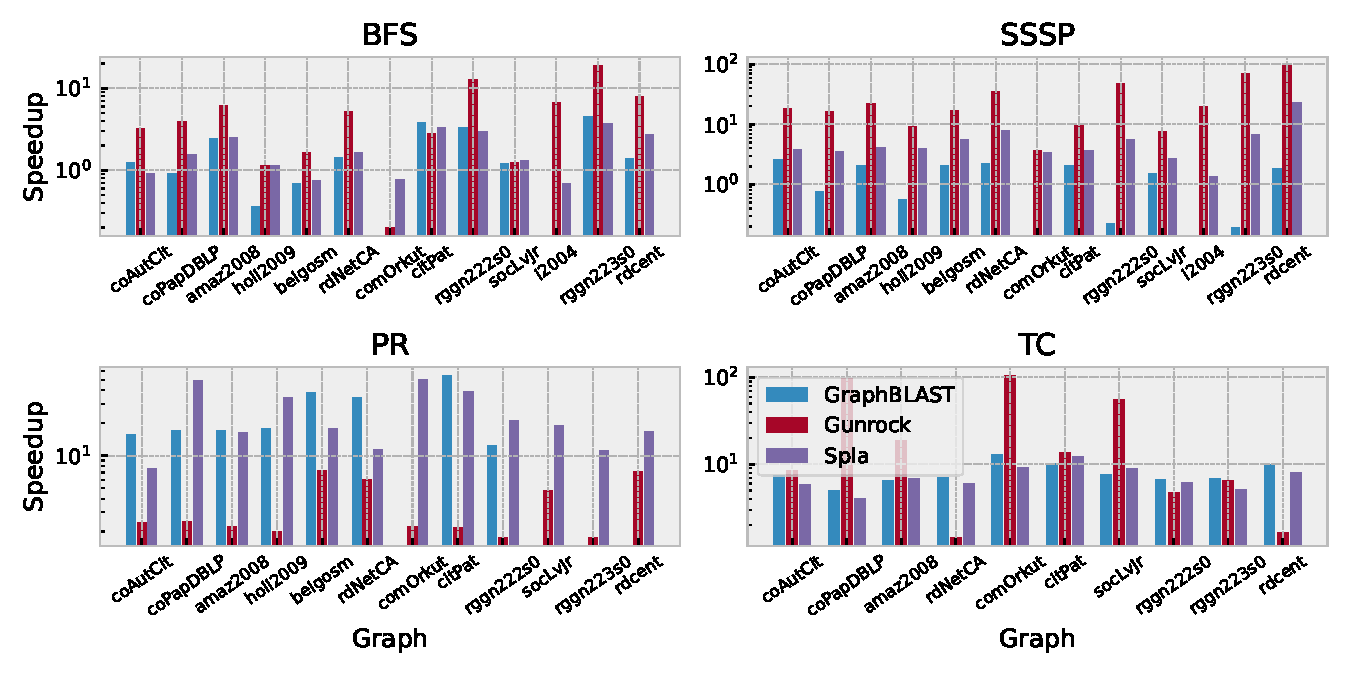
\includegraphics[width=1.0\linewidth]{plots/rq1_rel.pdf}
\caption{Performance of Spla library and GPU tools on the same device, shown as a speedup relative to LaGraph. Logarithmic scale is used.}
\label{fig:rq1_chart}
\end{figure}

\begin{figure}[tbp]
\centering
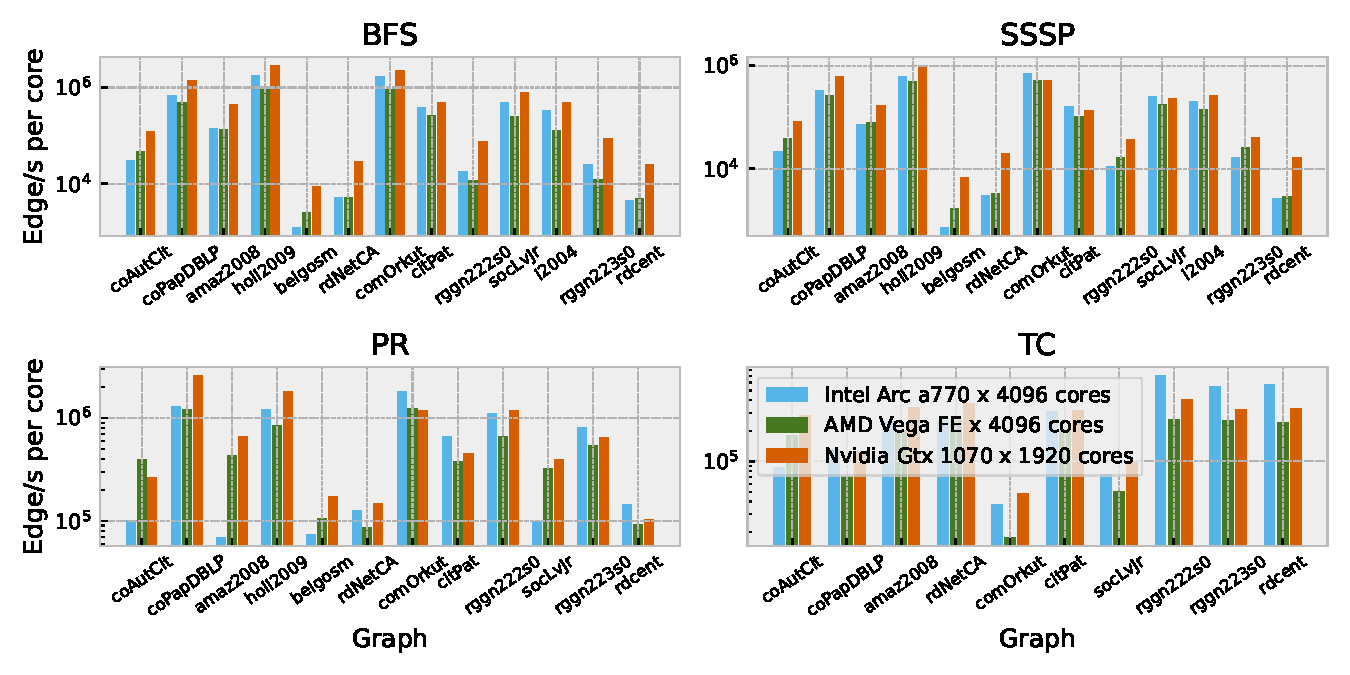
\includegraphics[width=1.0\linewidth]{plots/rq2_cores.pdf}
\caption{Performance of Spla library on different devices, shwon as edge/s througput per device core. Logarithmic scale is used.}
\label{fig:rq2_chart}
\end{figure}

\textbf{RQ1.} \textit{What is the performance of the proposed solution relative to existing tools for GPU analysis?} Taking a look at Fig.~\ref{fig:rq1_chart}, Spla shows very acceptable performance in all algorithms, running with comparable speed to its nearest competitor, GraphBLAST. Also proposed library does not suffer from memory issues on some large graphs. Spla is consistently several times faster than LaGraph, overcoming it up to $25\times$ in some cases. Gunrock is the fastest GPU framework for analysis. It dominates the overall performance and only suffers in a PR algorithm.\\

\textbf{RQ2.} \textit{What is the performance of the proposed solution on various devices vendors and OpenCL runtimes?} Spla successfully launches and workes on the GPU of distinct vendors, including Intel, AMD and Nvidia. It shows promising performance and demonstrated scalability in relation to the number of computing cores. Fig.~\ref{fig:rq2_chart} depicts the edge/s throughput per a GPU core for all devices. This metric is quite predictable for the same graphs. This can be seen if one takes into account the overall shape of the figures for BFS, SSSP and PR as a whole.